% --- UNIVERSAL PREAMBLE BLOCK ---
\documentclass[11pt, aspectratio=169]{beamer}
\usepackage{geometry}
\usepackage{fontspec}

\usepackage[romanian]{babel}

% Set fonts
\setmainfont{Noto Sans}
\setsansfont{Noto Sans}
\setmonofont{Noto Sans Mono}

% Beamer Theme Settings
\usetheme{Madrid}
\usecolortheme{default}
\setbeamertemplate{navigation symbols}{} % Remove navigation symbols for a cleaner look

% Document Information
\title[TranceVR]{TranceVR: De la Dungeon Procedural la Randare Fractală în WebXR}
\subtitle{Studiu de caz: optimizare, eșecuri tehnice și procesare de semnal}
\author{Buciu Theodor, Țacu Darius Ștefan}
\date{\today}

\begin{document}

% Slide 1: Title
\begin{frame}
    \titlepage
\end{frame}

% Slide 2: Eșecul #1 – Babylon.js Editor
\begin{frame}{Eșecul \#1 – Babylon.js Editor}
    \begin{itemize}
        \item \textbf{Ipoteză:} Utilizarea editorului vizual (Babylon.js Editor) pentru compoziția rapidă a scenei 3D.
        \item \textbf{Realitate:} Lipsă totală de optimizare pentru scene cu instanțieri complexe.
        \item \textbf{Problema (The 3 FPS Crash):} Overhead masiv în graful scenei. Fiecare nod vizual introducea latență, blocând Render Loop-ul.
        \item \textbf{Concluzie:} Editorul a fost abandonat complet. S-a decis trecerea la \textbf{Cod Pur (TypeScript)}
    \end{itemize}
\end{frame}

% Slide 3: Fundația Tehnică (Restart)
\begin{frame}{Fundația Tehnică (Restart)}
    \begin{itemize}
        \item \textbf{Motorul Core:} Utilizarea \texttt{@babylonjs/core} instanțiat manual, eliminând abstractizările inutile.
        \item \textbf{Fizica:} Integrarea motorului \textbf{Havok Physics} (librărie WASM ultra-performantă) pentru simularea precisă și rapidă a coliziunilor (Ground/Player).
    \end{itemize}
\end{frame}

% Slide 4: Eșecul #2 – Conceptul "Infinite Dungeon"
\begin{frame}{Eșecul \#2 – Conceptul "Infinite Dungeon"}
    \begin{columns}
        \begin{column}{0.5\textwidth}
            \begin{itemize}
                \item \textbf{Ideea:} Un coridor infinit creat procedural din 3-4 module realizate în Blender.
                \item \textbf{Mecanica:} Concatenare dinamică via \texttt{LevelStreamingSystem}.
                \item \textbf{Punctul critic:} Shadere audio-reactive aplicate direct pe pereții fizici.
                \item \textbf{Cauza eșecului:} Incompatibilitate între materialele PBR din `.glb` și injecția de cod GLSL vertex shader și pipeline-ul babyon.js. Scăderi drastice de framerate și artefacte vizuale (Z-fighting).
            \end{itemize}
        \end{column}
        \begin{column}{0.5\textwidth}
            \begin{figure}[htbp]
                \centering
                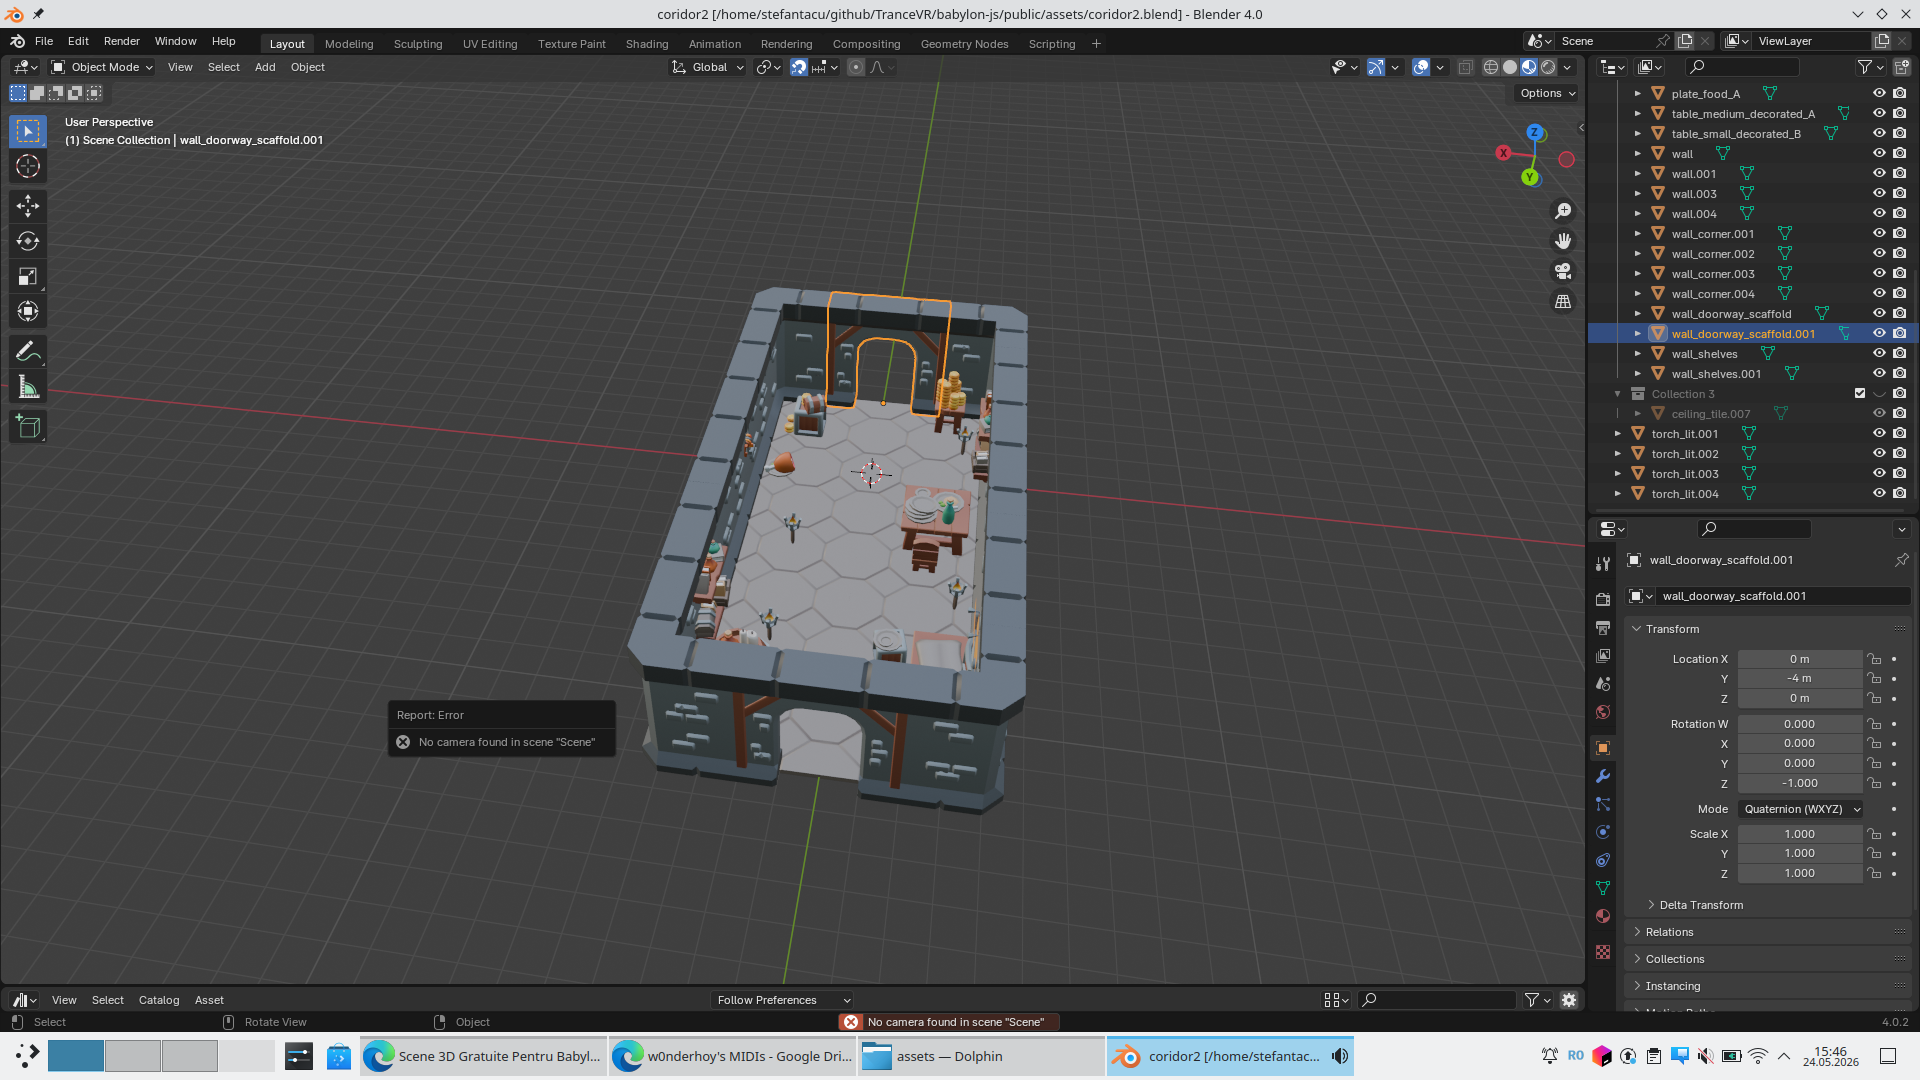
\includegraphics[width=0.9\textwidth]{images/corridor.png}
                \caption{Module Blender - Vedere top-down coridoare .glb}
            \end{figure}
        \end{column}
    \end{columns}
\end{frame}

% Slide 5: Pivotul Final – Minimalizarea Scenei
\begin{frame}{Pivotul Final – Minimalizarea Scenei}
    \begin{columns}
        \begin{column}{0.6\textwidth}
            \begin{itemize}
                \item \textbf{Decizie Arhitecturală:} Abandonarea coridoarelor geometrice și a sistemului de streaming.
                \item \textbf{Noua Viziune:} O singură cameră VR într-un spațiu infinit, generat matematic pe ecran.
                \item \textbf{Design "Ochelari de Cal":} Randăm totul intr-ul fragment shader (Fractal Raymarching), eliminând complet geometria 3D tradițională.
                \item \textbf{Mecanica Vizuală:} Trecerea la un \textbf{Global Screen-Space Shader}. Elimină definitiv problemele de adâncime și costurile de instanțiere.
            \end{itemize}
        \end{column}
        \begin{column}{0.4\textwidth}
            \begin{figure}[htbp]
                \centering
                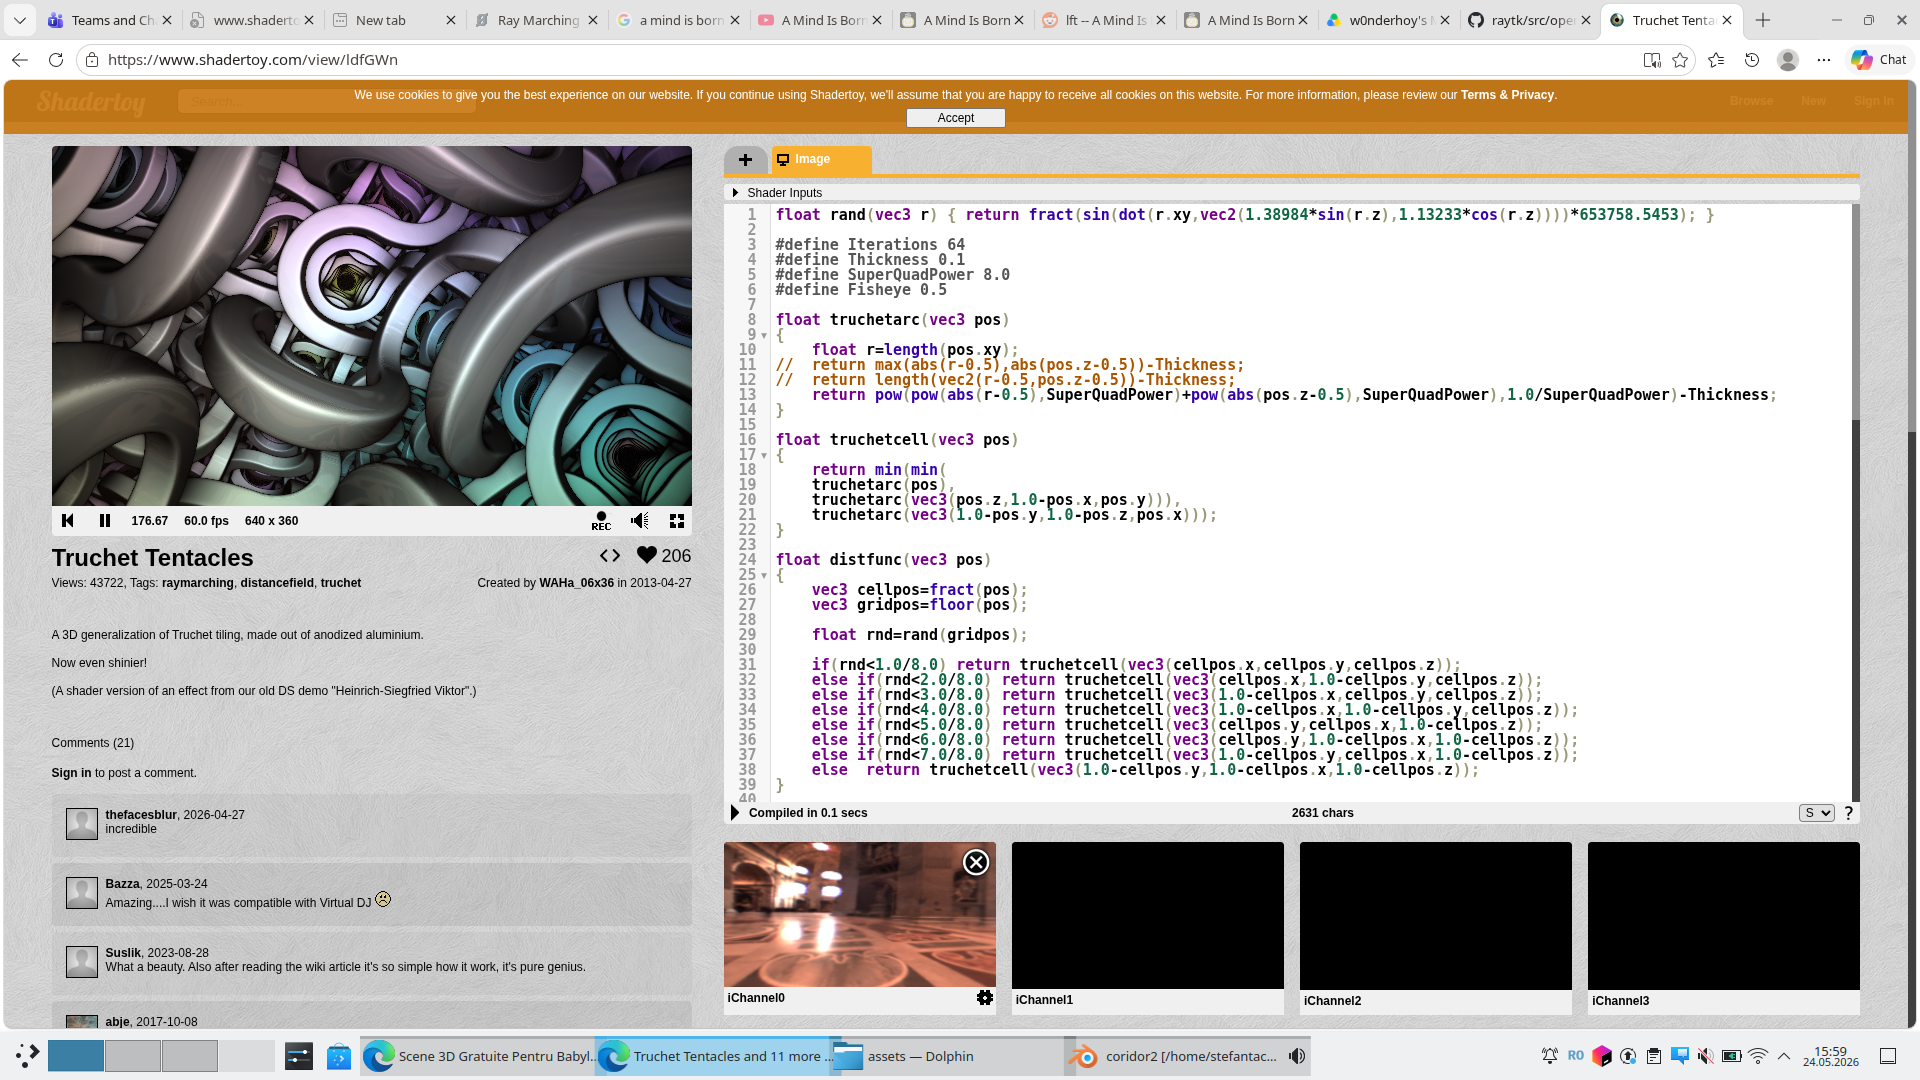
\includegraphics[width=\textwidth]{images/shader.png}
                \caption{Rezultat Final: Shader Fractal Reactiv}
            \end{figure}
        \end{column}
    \end{columns}
\end{frame}

% Slide 6: Analiza Spectrală – Deep Dive în FFT
\begin{frame}{Analiza Spectrală – Deep Dive în FFT}
    \begin{itemize}
        \item \textbf{Tehnologie:} Web Audio API (\texttt{AnalyserNode}) integrat în \texttt{AudioService}.
        \item \textbf{Fast Fourier Transform (FFT):} Transformarea semnalului din domeniul timpului în frecvență. Rezoluție: 512 unități (bins).
        \item \textbf{Smoothing:} Factor de $0.6$ pentru a evita efectul obositor de "flicker" vizual.
        \item \textbf{Extracția Semantică a Benzilor (Feature Extraction):}
              \begin{itemize}
                  \item \textbf{BASS ($\sim$0-250 Hz):} Controlează macro-structura și "Kick-ul" ($\sim$0-170 Hz).
                  \item \textbf{MID ($\sim$250-2000 Hz):} Influențează densitatea vizuală.
                  \item \textbf{TREBLE / HIGH ($\sim$2000+ Hz):} Direcționează efectele ascuțite (Snare, Glitch).
              \end{itemize}
    \end{itemize}
\end{frame}

% Slide 7: Shader-ul Fractal Reactiv
\begin{frame}{Shader-ul Fractal Reactiv (GLSL)}
    \begin{itemize}
        \item \textbf{Implementare:} Fragment Shader injectat prin \texttt{FractalPostProcessService}.
        \item \textbf{Comunicarea CPU-GPU (Uniforms):}
              \begin{itemize}
                  \item \texttt{uBass}, \texttt{uTreble}, \texttt{uKick}: Valori trimise la fiecare cadru (Render Loop) direct din analiza FFT.
                  \item \texttt{uTime}: Pentru evoluția continuă a zgomotului matematic.
              \end{itemize}
        \item \textbf{Sursa de Inspirație:} Model matematic bazat pe \url{https://www.shadertoy.com/view/ldfGWn}
        \item \textbf{Suport WebXR Nativo:}
              \begin{itemize}
                  \item În modul stereoscopic (VR), fiecare ochi primește o randare corectă.
                  \item Utilizarea \texttt{uInverseViewProj} (Matricea inversă de View-Projection) pentru a alinia proiecția fractală cu mișcările capului (6DoF).
              \end{itemize}
    \end{itemize}
\end{frame}

% Slide 8: Concluzii – Lecții de Development
\begin{frame}{Concluzii – Lecții de Development}
    \begin{itemize}
        \item \textbf{Performanța primează în XR:} Trecerea de la 3 FPS (Editor, Geometrie complexă) la stabilizarea la 75 FPS prin abordarea "Code-First" și mutarea calculelor grele în Fragment Shader.
        \item \textbf{Modularitate ECS:} Dezactivarea \texttt{LevelStreamingSystem} s-a putut face printr-o singură linie de cod (\texttt{enabled = false}) datorită arhitecturii decuplate.
    \end{itemize}
\end{frame}

% Slide 9: Sound Design – Patch-ul de Pure Data (Pd)
\begin{frame}{Sound Design – Patch-ul de Pure Data (Pd)}
    \begin{columns}
        \begin{column}{0.5\textwidth}
            \begin{itemize}
                \item \textbf{Dezvoltare Paralelă:} Crearea unui sintetizator custom utilizând mediul vizual de programare audio \textbf{Pure Data}.
                \item \textbf{Procesarea Semnalului:}
                      \begin{itemize}
                          \item Preia date brute din fișiere \texttt{.mid}.
                          \item Transformă trigger-ele MIDI într-un spectru de sunet cromatic.
                      \end{itemize}
                \item \textbf{Integrarea în Babylon.js:} Sunetul generat procedural a fost înregistrat și exportat (.wav/.mp3), asigurând o corelație matematică perfectă cu \texttt{AnalyserNode}.
            \end{itemize}
        \end{column}
        \begin{column}{0.5\textwidth}
            \begin{figure}[htbp]
                \centering
                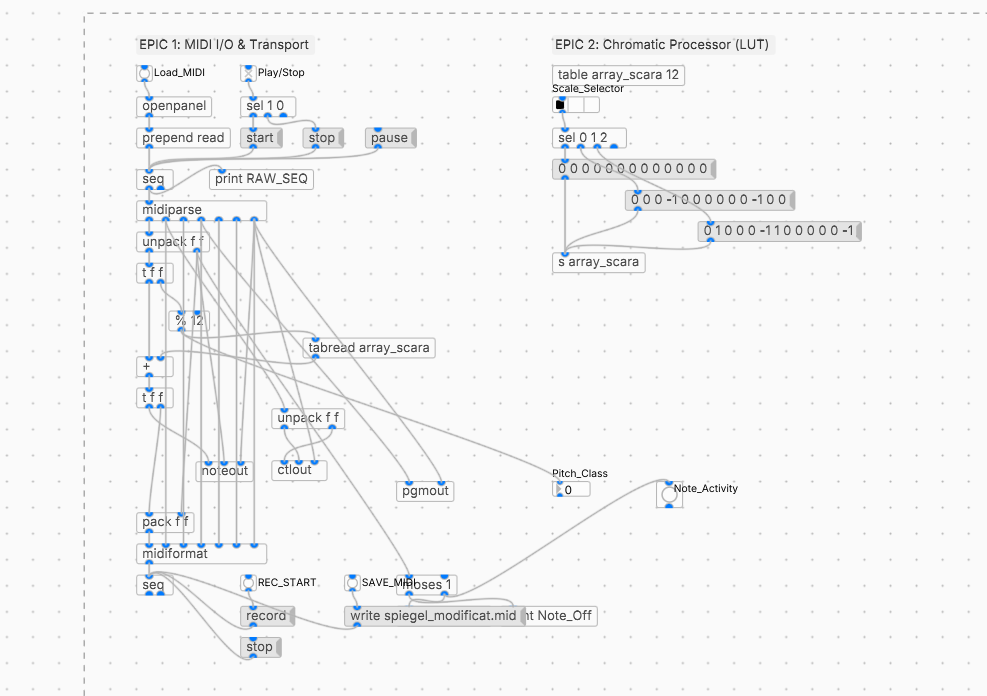
\includegraphics[width=0.9\textwidth]{images/patch-pd.png}
                \caption{Interfața Pure Data - Patch de Sinteză}
            \end{figure}
        \end{column}
    \end{columns}
\end{frame}

% Slide 10: Q&A
\begin{frame}
    \begin{center}
        \Huge \textbf{Vă mulțumesc!} \\[1cm]
        \Large Întrebări?
    \end{center}
\end{frame}

\end{document}
